% =============================================================================
\section{Simulation Environment (\texttt{lily\_gz})}
\label{sec:sim}
% =============================================================================

\begin{center}
\noteto{Francisco}{This section please -- I've trimmed it down a lot: no need to get into ROS~2/bridging/topic-plumbing details here, that's covered structurally elsewhere. Focus this section on the Gazebo environment itself (worlds, assets) and the wave/wind plugins used to make it a realistic ASV testbed. Please also add pictures/screenshots of the simulated worlds and, if applicable, the wave/wind effects in action.}
\end{center}

\subsection{Overview}

The digital twin runs on \textbf{Gazebo Harmonic}, reusing several assets originally developed for VRX (the RobotX/VRX surface-vehicle simulation suite): buoys, docks, and land-block obstacles. \texttt{lily\_environment.launch.py} is config-driven -- it takes a \texttt{world} launch argument (e.g.\ \texttt{alqueva}, \texttt{viana}, \texttt{viana\_buoys}, \texttt{feup}, \texttt{empty}) and loads the corresponding \texttt{.sdf} world file, along with the models and per-world spawn poses that populate it.

\subsection{Environmental plugins: waves and wind}

\todored{Describe here the Gazebo plugins used to model the water surface (wave field: amplitude/period/direction, whether it produces visual-only waves or also hydrodynamic forcing on the hull) and wind (constant or gusting wind field, force/torque applied to the hull and any exposed superstructure). Note which worlds/missions had these environmental effects enabled versus running in calm/no-wind conditions, and whether the reported results (Section~\ref{sec:results}) were obtained with them on or off.}

\subsection{Vehicle model and worlds}

The \texttt{lily} Gazebo model (\texttt{lily\_gz/models/lily/model.sdf}) uses dedicated hull/housing/mount/propeller meshes and PBR textures. Five worlds are checked in: \texttt{empty} (unit testing), \texttt{feup} (campus pond, used for the square mission), \texttt{alqueva} and \texttt{viana}/\texttt{viana\_buoys} (larger reservoir/coastal environments, the latter with spawned red/dummy buoys for perception-in-the-loop testing), and \texttt{dynamic\_world} (\todored{describe the purpose of \texttt{dynamic\_world.sdf} -- e.g.\ moving obstacles/waves -- if used for the reported results}).

\begin{figure}[H]
\centering
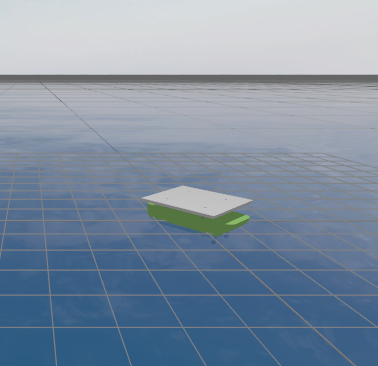
\includegraphics[width=0.6\linewidth]{figures/lily_gazebo.png}
\caption{The \texttt{lily} vehicle model floating in the Gazebo Harmonic simulation, showing the hull and deck meshes on the water surface.}
\label{fig:sim_world}
\end{figure}
